\chapter[\emph{Refactoring}: Modernizando feets]{
    \emph{Refactoring}: Modernizando \acrshort{feets}
}
\label{chapter:refactoring}

Además de paralelizar la extracción de características, con la nueva versión de \gls{feets} llevamos a cabo un proceso de refactorización que buscó modernizar el diseño general del sistema, proporcionar una \gls{api} más simple e intuitiva, y mejorar aún más el desempeño de los extractores. Este proceso de reingeniería, a su vez, dio lugar a la actualización del \emph{stack} tecnológico de la aplicación, la estandarización del estilo del código a lo largo y ancho del proyecto, y también al desarrollo de nuevas funcionalidades que consideramos útiles.

En las siguientes secciones del capítulo describiremos en detalle cada una de las modificaciones que implementamos en la nueva versión de \gls{feets}. Haremos hincapié en las decisiones de diseño que tomamos durante el proceso de desarrollo, y también hablaremos de las actualizaciones tecnológicas que llevamos a cabo en la infraestructura del proyecto.  

\section{Rediseño de extractores}

Uno de los cambios más importantes entre la versión original de \gls{feets} y la nueva implementación fue la completa renovación de la lógica de los extractores de características. El cambio consistió en volver a implementar la clase \texttt{Extractor} desde cero, que funciona como el modelo base detrás de todos los extractores del sistema.

La problemática que impulsó el rediseño de los extractores fue la complejidad que manejaba la metaclase \texttt{Extractor} la cual, como se explicó en el capítulo \autoref{chapter:feets}, mantenía una lógica compleja con uso de metaprogramación avanzada para asegurar el correcto comportamiento de las clases hijas. Tales técnicas estaban destinadas a asegurar que todas estas clases siguieran una interfaz común, definiendo métodos y atributos que deben ser implementados por todos los extractores y realizando validaciones específicas al momento de ejecución para verificar que el comportamiento sea el correcto.

En la nueva versión, reimplementamos desde cero la clase \texttt{Extractor} reemplazando el uso de la metaclase por el de una clase abstracta. Al igual que con la metaclase, esto nos permite especificar métodos y atributos obligatorios en la interfaz, pero lo hace de una manera más simple y fácil de entender sin la necesidad de técnicas de metaprogramación, buscando reducir drásticamente la complejidad de la clase. 

Además de emplear el uso de una clase abstracta, aprovechamos la reimplementación de la clase \texttt{Extractor} para también agregar nuevas funcionalidades a la interfaz y para eliminar algunos atributos redundantes. Las modificaciones se pueden visualizar en la figura \autoref{fig:extractor_class}, que compara los diagramas de clase de los extractores entre las versiones original y nueva de \gls{feets}.

\begin{figure}[!ht]
\centering
\begin{subfigure}{\textwidth}
    \centering
    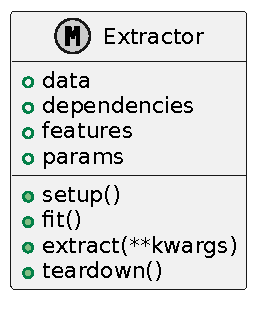
\includegraphics[width=.25\linewidth]{07_refactoring/figures/extractor_old.pdf}
    \caption{Diagrama de clases original}
\end{subfigure}

\begin{subfigure}{\textwidth}
    \centering
    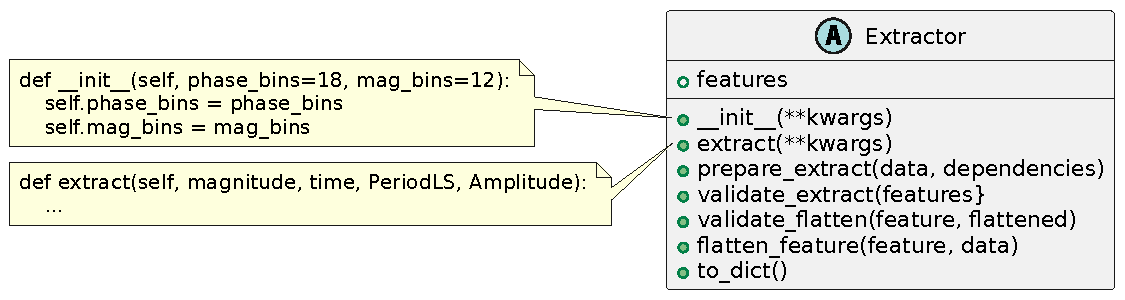
\includegraphics[width=\linewidth]{07_refactoring/figures/extractor_new.pdf}
    \caption{Nuevo diagrama de clases.}
\end{subfigure}

\caption{
    Diagramas de clase de \texttt{Extractor} antes y después de la nueva versión de \gls{feets}. Las anotaciones de la izquierda ejemplifican posibles implementaciones de los métodos señalados.
}
\label{fig:extractor_class}
\end{figure}

A continuación, hablaremos más en detalle sobre las distintas modificaciones que realizamos en la \gls{api} de extractores.

\begin{description}
    \item[Método de extracción] En primer lugar, los métodos \texttt{fit()} y \texttt{extract()} fueron reemplazados por un solo método abstracto, también con el nombre \texttt{extract()}, el cual debe ser implementado por todos los extractores con la lógica de extracción correspondiente.
    
    Los argumentos de entrada consisten de
    \begin{itemize}
        \item los vectores de datos de la \gls{lc} utilizados en el cálculo de las características,
        
        \item las características computadas por otros extractores que actúan como dependencias.
    \end{itemize}
    Cada uno de estos argumentos puede o bien ser obligatorio, requerido para la extracción; o ser opcional, con valores por defecto.

    \item[Método de inicialización] A diferencia de \texttt{fit()}, el nuevo método \texttt{extract()} no cuenta con parámetros extra para configuraciones opcionales. Esto es porque los parámetros de un extractor ya no se pasan como argumentos en el momento de su ejecución, sino que se asignan como atributos de la instancia durante la inicialización del objeto. 
    
    Ahora se permite la implementación de un método opcional \texttt{\_\_init\_\_()} personalizado en cada clase, el cual toma como argumentos de entrada los valores de los parámetros opcionales del extractor y los asigna a atributos de la clase durante su inicialización. Como requerimiento, los parámetros de un extractor son todos opcionales, por lo que se deben especificar en forma de \emph{keyword arguments} con valores por defecto.

    \item[Atributos redundantes] A simple vista es fácil notar que los atributos \texttt{data}, \texttt{dependencies} y \texttt{params} ya no se especifican en el cuerpo de la clase. Esto es porque todos estos valores se infieren automáticamente a partir de los argumentos que se especificaron en los nuevos métodos:

    \begin{itemize}
        \item Del método \texttt{\_\_init\_\_()} es posible determinar los parámetros opcionales del extractor (\texttt{params}).
        \item Los argumentos de \texttt{extract()} hacen posible inferir los datos de la \acrfull{lc} requeridos por el extractor (\texttt{data}), así como las dependencias de características (\texttt{dependencies}).
    \end{itemize}

    La inferencia de estos atributos se logra mediante introspección, una técnica de metaprogramación que permite al programa examinar su propia estructura en tiempo de ejecución. En este caso, se aplica en el momento de definición de la clase, permitiendo realizar validaciones y asegurar que los atributos inferidos respeten los formatos requeridos.

    \item[Normalización de características] Entre las nuevas funcionalidades de los extractores, incorporamos el método \texttt{flatten\_feature()} para normalizar las características computadas a valores unidimensionales. En particular, el método permite transformar diccionarios, listas o vectores de \emph{Numpy} a colecciones de valores escalares, de una sola dimensión.
    
    En caso de tratar con valores que no estén dentro de los tipos de datos soportados, el usuario puede expandir la lógica de este método en el extractor correspondiente para agregar la transformación adecuada para el tipo de datos necesario.

    \item[Persistencia] Con la intención de persistir el estado de los extractores entre ejecuciones, agregamos el método \texttt{to\_dict()} que provee una representación del estado interno del extractor en forma de un diccionario de Python. El diccionario incluye el nombre del extractor y los valores de los parámetros opcionales que se le asignaron al momento de incialización.

    \item[Método auxiliares] Por último, incorporamos algunos métodos destinados a acompañar comportamientos internos en la aplicación:

    \begin{itemize}
        \item \textbf{\texttt{prepare\_extract()}}: Confecciona y valida los argumentos del método \texttt{extract()} a partir de una selección de vectores de datos y de dependencias de características.
        \item \textbf{\texttt{validate\_extract()}}: Valida que la salida de  \texttt{extract()} produzca las características esperadas.
        \item \textbf{\texttt{validate\_flatten()}}: Valida que la salida de \texttt{flatten\_feature()} tenga el formato de una característica normalizada.
    \end{itemize}
\end{description}

El nuevo comportamiento de los métodos \texttt{extract()} e \texttt{\_\_init\_\_()}, así como la eliminación de definiciones de atributos \texttt{data}, \texttt{dependencies} y \texttt{params} del cuerpo de la clase, significó cambios mayores en la infraestructura de los extractores, lo que nos llevó a actualizar todos los extractores ya desarrollados en \gls{feets} para que adopten los nuevos requerimientos, y para que no rompan el comportamiento ya existente de la aplicación.

\section{Integración con \emph{LightCurve}}

En nuestra búsqueda por hacer que \gls{feets} sea más rápido, decidimos integrarla con una de las herramientas más modernas en la extracción de características de series temporales: \emph{LightCurve}. Desarrollada por \citet{malanchev2021lightcurve}, esta biblioteca se distingue por su enfoque en la eficiencia computacional, logrando tiempos de ejecución considerablemente menores en comparación con implementaciones tradicionales en Python. 

El secreto detrás de esta mejora radica en su implementación en Rust, un lenguaje de programación de bajo nivel diseñado para ofrecer alto rendimiento, pero sin comprometer la seguridad ni la concurrencia del código \citep{matsakis2014rust}. Rust permite ejecutar operaciones numéricas de forma optimizada, aprovechando técnicas avanzadas de paralelización y un uso eficiente de la memoria. Gracias a esto, \emph{LightCurve} supera muchas de las limitaciones de los extractores originales de \gls{feets}, proporcionando una ejecución más rápida y escalable, especialmente en el procesamiento de grandes volúmenes de datos.

En esta nueva versión, incorporamos todas las características de \emph{LightCurve} en \gls{feets}. Esto no solo amplía la lista de extractores disponibles para el análisis de series temporales, sino que también nos permitió reemplazar extractores preexistentes por sus versiones más eficientes, de lo posible. Así, en lugar de reinventar lo que ya está optimizado, optamos por una integración inteligente que nos permite combinar la flexibilidad de \gls{feets} con la velocidad de \emph{LightCurve}, logrando así lo mejor de ambos mundos.

Para hacer la integración lo más transparente posible, desarrollamos una nueva clase abstracta: \texttt{LightCurveExtractor}. Esta clase extiende el diseño de los extractores originales de \gls{feets} actuando como un puente entre ambas bibliotecas. A través de esta interfaz, cualquier extractor basado en \emph{LightCurve} se adapta automáticamente a la arquitectura de \gls{feets}, sin necesidad de cambios manuales ni configuraciones adicionales.

Uno de los principales desafíos en esta integración fue la diferencia en la representación de datos entre ambas bibliotecas. Mientras que \gls{feets} trabaja tradicionalmente con magnitudes aparentes, muchos de los extractores de \emph{LightCurve} operan directamente sobre flujos. El flujo es una medida física fundamental en astronomía, que representa la cantidad de luz recibida de un objeto en una determinada banda espectral y que, en muchos contextos, es más adecuada que la magnitud para ciertos tipos de análisis \citep{bessell2005standard}. Para hacer frente a esta diferencia, introdujimos dos nuevos tipos de datos en \gls{feets}, \texttt{flux} y \texttt{flux\_error}, asegurando así que los extractores de ambas bibliotecas puedan coexistir sin problemas dentro de la misma plataforma.

\section[Mejoras en la API]{
    Mejoras en la \gls{api}
}

Acompañando la reimplementación de los extractores, también incorporamos modificaciones en la \gls{api} del \texttt{FeatureSpace} para ofrecer nuevas funcionalidades a la herramienta y mejorar la flexibilidad de la extracción de características. Todas estas mejoras se detallan a continuación.

\begin{description}
    \item[Grupos de \acrlongplsp{lc}] Una de las principales molestias en el uso de \gls{feets} era que solo se podían extraer las características de una sola \gls{lc} a la vez. Bajo este modelo, si se querían analizar las mismas características entre varias \glspl{lc} distintas, hacía falta crear múltiples instancias de \texttt{FeatureSpace}, todas con la misma selección de características a extraer. Este proceso no solo puede ser tedioso si se quiere trabajar con varias curvas diferentes, sino que además puede llevar a inconsistencias cuando el usuario modifica la selección de uno de los tantos \texttt{FeatureSpace} inicializados y no tiene la consideración de realizar el mismo cambio en las demás instancias.
    
    Por esto, en la nueva versión de \gls{feets}, dimos soporte al procesamiento de múltiples \glspl{lc} en simultáneo mediante la instanciación de un único \texttt{FeatureSpace}, el cual define los conjuntos de características que se desean extraer para todas las curvas especificadas. 

    Aprovechando también la nueva implementación paralelizada del proceso de extracción, decidimos hacer que la ejecución de las distintas \glspl{lc} también sea paralelizada, por lo que no solo se reduce la cantidad de instancias de \texttt{FeatureSpace} que debe manejar el usuario, sino que además se aprovechan los recursos disponibles en el sistema para mejorar aún más el desempeño temporal de la aplicación. 
    
    \item[Selección automática de características] Otro de los cambios que implementamos fue una mejora al proceso de selección de características que ocurre previo al flujo de extracción. Para ser más específicos, incorporamos una nueva forma de inicializar el \texttt{Fea\-ture\-Space} que, partiendo de una \gls{lc}, permite seleccionar automáticamente todas las características que se pueden extraer a partir de los vectores de datos disponibles en la curva.
    
    El nuevo constructor, \texttt{from\_lc()}, funciona también para el caso en que se desea procesar más de una \gls{lc} a la vez. En este escenario, nos aseguramos que la selección final consista únicamente de las características extraíbles por todas las \glspl{lc} proporcionadas, teniendo en consideración que las distintas curvas no necesariamente presentan los mismos vectores de datos.
    
    Esta funcionalidad es muy útil porque facilita tremendamente la selección de todas las características posibles. Antes de este cambio, el usuario debía revisar las dependencias de datos de todos los extractores del sistema para determinar qué características eran alcanzables por la curva trabajada mientras que, en la nueva versión, todo este proceso se resuelve automáticamente con la llamada a un único método.

    \item[Persistencia de estados] Consideramos necesario el contar con un mecanismo para almacenar y reutilizar las configuraciones específicas de la extracción de características, por lo que añadimos la capacidad de exportar e importar objetos de la clase \texttt{FeatureSpace}.
    
    En la nueva interfaz, los usuarios son capaces de guardar instancias de un \texttt{FeatureSpace} en forma de diccionarios de Python o como archivos en los formatos \emph{JavaScript Object Notation} (JSON) \citep{bray2014json} o \emph{YAML Ain't Markup Language} (YAML) \citep{ben2009yaml}; todo esto, mediante los nuevos métodos \texttt{to\_dict()}, \texttt{to\_json()} y \texttt{to\_yaml()}, respectivamente. 
    
    A partir de las estructuras exportadas, los usuarios pueden hacer uso de los constructores \texttt{from\_dict()} (para diccionarios), \texttt{from\_json()} (archivos JSON) y \texttt{from\_yaml()} (archivos YAML), que les permiten restaurar el estado del \texttt{FeatureSpace} original con todas las configuraciones guardadas. Estos estados incluyen las características seleccionadas para ser extraídas, las instancias parametrizadas de los extractores, los datos requeridos por la selección de características, y algunas opciones particulares para ajustar la extracción paralelizada.
    
    La gestión de las tareas de lectura y escritura de archivos las desarrollamos en un nuevo módulo del sistema, \texttt{io}, quien además se encarga de la correcta codificación de las configuraciones a los distintos formatos permitidos.

    \item[Interfaz de características] Por último, otra de las principales mejoras de la \gls{api} fue la introducción de la clase \texttt{Features}, que redefine la forma en que se exploran los resultados de la extracción de características. Con una interfaz más robusta y una funcionalidad expandida, \texttt{Features} viene a reemplazar la clase \texttt{FeatureSet}, implementada en la versión original de \gls{feets}.

    El objetivo principal de la clase \texttt{Features} es el de manejar la representación de las características resultantes del procesamiento de una o varias \glspl{lc} para su análisis posterior. Una instancia de esta clase se puede explorar de dos formas distintas:
    \begin{itemize}
        \item como un arreglo de \glspl{lc}, donde cada elemento consiste de un diccionario con los resultados de todas las características de una de las curvas procesadas; o bien,
        \item como un objeto, en el que cada atributo representa una de las características seleccionadas, y su valor es un arreglo con los respectivos resultados obtenidos en cada \gls{lc}.
    \end{itemize}

    Con la intención de usar esta clase para el análisis de características, implementamos también la capacidad de representar los datos en forma de un \texttt{DataFrame} de \emph{Pandas}\footnote{\url{https://pandas.pydata.org/}}, mejorando también la interoperabilidad de \gls{feets} dentro del ecosistema de Python. Con esto en mente, la clase \texttt{Features} puede servir como base para futuras herramientas de análisis, aprovechando su estructura actual para modelar, por ejemplo, una forma de proporcionar un gráfico representativo de cada característica.
\end{description}

    \section{Cambios menores}

Además de las mejoras fundamentales introducidas en esta nueva versión de \gls{feets}, realizamos una serie de optimizaciones y actualizaciones que elevan significativamente la calidad, compatibilidad y usabilidad del proyecto. Estos cambios, aunque menores en términos de implementación, impactan en la experiencia de los usuarios y en la eficiencia del código, asegurando que \texttt{feets} se mantenga alineado con las mejores prácticas y tecnologías más avanzadas. A continuación, detallamos las principales mejoras incorporadas:

\begin{description}
    \item[Compatibilidad] Actualizamos los requisitos de \gls{feets} y eliminamos por completo el soporte para Python 2. Ahora, \texttt{feets} es compatible con las versiones de Python 3.10 a 3.13 inclusive, lo que permite aprovechar las últimas optimizaciones y nuevas características del lenguaje.

    Entre las novedades más destacadas, Python 3.13 introduce un modo de ejecución experimental sin el \acrfull{gil}, haciendo opcional su uso y permitiendo \emph{full-threading} en escenarios altamente paralelizables \citep{gross2023nogil}. Si bien esta funcionalidad aún está en sus primeras etapas, su desarrollo representa un cambio radical en la evolución del lenguaje y abre nuevas posibilidades para mejorar el rendimiento de bibliotecas científicas y de análisis de datos. A medida que esta tecnología madure en futuras versiones, \texttt{feets} estará preparado para aprovechar todo su potencial.

    \item[Actualización de bibliotecas] En la nueva versión, renovamos por completo las dependencias principales para garantizar estabilidad, seguridad y acceso a las últimas innovaciones en \emph{Data Science}. Destacan particularmente las mejoras introducidas en:
    \begin{itemize}
        \item \emph{AstroPy} 7.0, que incorpora múltiples optimizaciones en el manejo de datos astronómicos, nuevas herramientas para análisis de series temporales y un rendimiento significativamente mejorado en operaciones comunes \citep{astropy2013astropy, astropy2018astropy, astropy2022astropy}.
        \item \emph{NumPy} 2.2.0, que introduce mejoras sustanciales en la eficiencia de operaciones matriciales, reducción del consumo de memoria y una mejor integración con las últimas versiones de Python \citep{harris2020array}. Estas optimizaciones son fundamentales para el procesamiento de grandes volúmenes de datos en \texttt{feets}, mejorando la velocidad de extracción de características sin comprometer la precisión.
    \end{itemize}

    \item[Estilo del código] La legibilidad y la calidad del código son fundamentales en un proyecto de código abierto, por lo que reforzamos el cumplimiento del estándar PEP 8 \citep{van2001pep8} y automatizamos el ajuste del formato con herramientas especializadas. Utilizamos:
    \begin{itemize}
        \item \emph{Flake8}\footnote{\url{https://flake8.pycqa.org/en/latest/}}, para garantizar un análisis estático del código y detectar posibles errores antes de su ejecución.
        \item \emph{Black}\footnote{\url{https://black.readthedocs.io/en/stable/}}, para asegurar un estilo consistente, facilitando la lectura del código y simplificando la colaboración entre varios desarrolladores.
    \end{itemize}

    \item[Ampliación de documentación y \emph{testing}] Para garantizar que los usuarios puedan aprovechar al máximo las nuevas capacidades de \texttt{feets}, expandimos y refinamos la documentación oficial de la herramienta. Ahora incluye ejemplos prácticos de uso, mejores explicaciones sobre la estructura de la \gls{api} y un tutorial actualizado con las nuevas funcionalidades incorporadas.

    Además, revisamos y actualizamos la \emph{test suite} para reflejar todos los cambios en la \gls{api}, asegurando una cobertura completa de las nuevas funcionalidades. Esta estrategia no solo mejora la confiabilidad del software, sino que también facilita futuras expansiones del proyecto sin comprometer la estabilidad del código base.
\end{description}